\section{Análise de Sistema de Arquivos}
    
    \vspace{10.5cm}
    
    \hspace{1cm}
    Neste capítulo, abordaremos algumas técnicas e ferramentas para coleta e análise de dados oriundos de máquinas investigadas. Como revisado na seção \ref{cap1_visao_geral_sa}, sistemas de arquivos são responsáveis por manter as abstrações de arquivo e diretório para o usuário final. Consequentemente, quando estamos investigando um sistema, é possível descobrir o que estava sendo usado nele, à medida que vestígios digitais são coletados e analisados.
    
    \subsection{Técnicas}
    
    \hspace{1cm}
    Antes de analisar os dados de um sistema, é preciso coletá-los. Tal operação consiste em gerar pelo menos duas cópias dos dados: a original e aquela que será usada pelo perito. Além disso, deve-se manter a integridade dos dados para eles configurarem evidências no futuro. Existem duas técnicas principais para coleta de dados: Coleta Lógica e Coleta \textit{bit-a-bit}.
    
    \subsubsection{Coleta Lógica}
    
    \hspace{1cm}
    Na coleta lógica, o profissional realiza uma cópia de arquivos e diretórios de um volume lógico, mas, essa cópia não inclui arquivos apagados e blocos de dados não utilizados \cite{kent2006}.
    
    \subsubsection{Coleta \textit{bit-a-bit}}
    
    \hspace{1cm}
    De outra forma, pode ser que o profissional necessite de uma cópia exata de todo o sistema de arquivos de um sistema-alvo. Para isso, ele dispõe da técnica de coleta \textit{bit-a-bit} para copiar os dados de um disco de armazenamento, seja para outro disco, seja para um novo arquivo \cite{kent2006}.
    
    \vspace{4mm}
    
    \hspace{1cm}
    Para garantir que os dados a serem coletados  não sejam modificados pelas ações do perito, emprega-se proteção contra escrita nas mídias encontradas. Como defende \citeonline{vecchia2019}, profissionais podem trabalhar com o \textit{Tableau} (figura \ref{tableau_img}).
    
    \begin{figure}[H]
    	\centering
    	\caption{Dispositivo de proteção contra escrita (Tableau)}
    	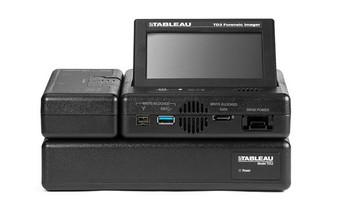
\includegraphics[scale=0.7]{img_tableau}
    	\caption*{Fonte: Google Imagens}
    	\label{tableau_img}
    \end{figure}
    
    \subsubsection{Análise de Dados}
    
    \hspace{1cm}
    Em dada investigação sobre um incidente, uma organização pode estar interessada em revelar quais arquivos foram usados por determinado empregado, e também quando isso ocorreu. Diante disso, o analista pode classificar arquivos por nome, metadados ou conteúdo, como sugere \citeonline{carrier2005}.
    
    \vspace{4mm}
    
    \hspace{1cm}
    O nome de um arquivo sugere o que ele pode tratar. Logo, ajuda em sua classificação. Os metadados fornecem informações como tempo de acesso e permissões dadas a algum usuário. O conteúdo de um arquivo pode ser útil, quando se busca uma palavra-chave ou formato específico.
    
    \subsection{Ferramentas} \label{cap2_ferramentas}
    
    \hspace{1cm}
    Existem ferramentas como \textit{dd} e \textit{Autopsy}, que podem nos ajudar a analisar dados de um SA. Enquanto a primeira gera um arquivo de saída com a cópia de um disco, a segunda interpreta a imagem gerada e tenta classificar as informações encontradas, para facilitar sua análise.
    
    \subsubsection{Programa \textit{dd}}
    
    \hspace{1cm}
    A ferramenta \textit{dd} é disponibilizada, por padrão, nas diversas distribuições Linux. Ela é usada para fazer cópia de arquivos em um formato especificado pelo usuário. Na coleta pericial, é possível replicar discos inteiros que estejam montados no sistema hospedeiro. Dessa forma, o perito pode gerar uma cópia de um disso num formato que a ferramenta Autopsy reconheça, como o formato E01.
    
    \subsubsection{Autopsy}

    \hspace{1cm}
    Emprega-se a Autopsy para realizar o exame dos dados coletados. Esta ferramenta fornece uma interface gráfica para que o perito opere os diversos utilitários da coleção de ferramentas de linha de comando Sleuth Kit.
    
    \vspace{4mm}
    
    \hspace{1cm}
    Por meio dos \textit{Ingest Modules}, esta ferramenta disponibiliza o recurso de análise automatizada de dados, para acelerar o processo de classificação de arquivos e diretórios de uma mídia de armazenamento. Sendo assim, o operador do programa pode navegar por uma árvore de arquivos enumerados semanticamente, para examinar o conteúdo de um sistema de arquivos.

    \subsection{Exercícios}
    
    \begin{example}[\quad \large Análise de Sistema de Arquivos] \label{cap2_exercicios}
        \begin{enumerate}
            \item Quais as técnicas de coleta de dados existem para examinar dados de sistemas de arquivos ?
            \item Qual a ferramenta, dentre aquelas apresentadas na seção \ref{cap2_ferramentas}, é ideal para um perito que queira replicar os dados de um disco ?
            \item Explique o motivo pelo qual se deve manter a integridade dos dados a serem analisados em uma investigação.
            \item Para que servem os \textit{Ingest Modules} da ferramenta \textit{Autopsy} ?
        \end{enumerate}
    \end{example}
    
\newpage